\section{Applicazioni}
\label{sec:Applicazioni}

Il programma riportato in \autoref{sec:Programma}, al seguito della creazione di una classe Python \cite{python_docs} rappresentante
la rete stradale studiata, può essere utilizzato per 3 diversi scopi:
\begin{itemize}
    \item Calcolo dell'equilibrio di Nash e del tempo di viaggio per le due popolazioni
    \item Calcolo dei grafici del tempo di viaggio e dell'equilibrio di Nash dipendenti dalla variazione dei costi delle strade
    \item Calcolo del grafico del tempo di viaggio e dell'equilibrio di Nash dipendenti dalla variazione delle popolazioni
\end{itemize}

\subsection{Paradosso di Braess}
\label{subsec:Es1}

Introduciamo la rete stradale così formata:
\[
\quad
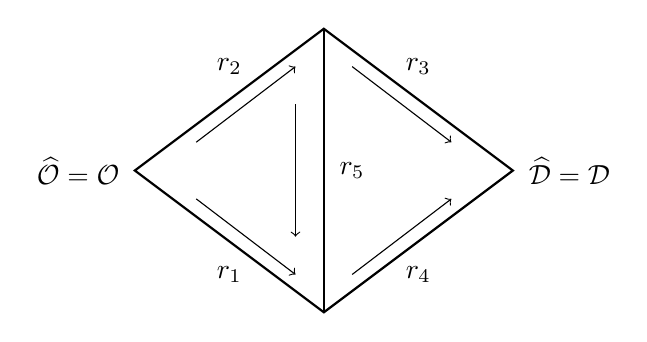
\begin{tikzpicture}[scale=1.2]

\coordinate (L) at (0,0);
\coordinate (T) at (2,1.5);
\coordinate (R) at (4,0);
\coordinate (B) at (2,-1.5);

\draw[thick] (L) -- (T) -- (R) -- (B) -- cycle;
\draw[thick] (T) -- (B);

\draw[->] (0.65,0.3) -- (1.7,1.1);

\draw[->] (0.65,-0.3) -- (1.7,-1.1);

\draw[->] (2.3,1.1) -- (3.35,0.3);

\draw[->] (2.3,-1.1) -- (3.35,-0.3);

\draw[->] (1.7, 0.7) -- (1.7, -0.7);

\node at (1,1.1) {$r_2$};
\node at (1,-1.1) {$r_1$};
\node at (3,1.1) {$r_3$};
\node at (3,-1.1) {$r_4$};
\node at (2.3, 0) {$r_5$};
\node at (-0.6, 0) {$\widehat{\mathcal{O}} = \widecheck{\mathcal{O}}$};
\node at (4.6, 0) {$\widehat{\mathcal{D}} = \widecheck{\mathcal{D}}$};
\end{tikzpicture}
\quad
\]
In prima analisi prendiamo l'esempio principe riguardante il Paradosso di Braess \cite{BraessParadox}, presente in svariati trattati sul tema (si veda, per esempio, \cite[Cap. 8]{Easley_Kleinberg_2010}).
Solitamente viene studiato con una singola popolazione sulla rete; nel nostro caso, riprendiamo i parametri utilizzati in \cite[Cap. 3]{MR4911797}:
\begin{equation*}
\begin{array}{r @{\hspace{2cm}} r}

\widehat{\tau}_1(\eta) = 45 &
\widecheck{\tau}_1(\eta) = 30 \\

\widehat{\tau}_2(\eta) = 40\widehat{\eta} &
\widecheck{\tau}_2(\eta) = 20\widecheck{\eta}+8\widehat{\eta} \\

\widehat{\tau}_3(\eta) = 45 &
\widecheck{\tau}_3(\eta) = 30 \\

\widehat{\tau}_4(\eta) = 40\widehat{\eta} &
\widecheck{\tau}_4(\eta) = 20\widecheck{\eta}+8\widehat{\eta} \\

\widehat{\tau}_5(\eta) = 0 &
\widecheck{\tau}_5(\eta) = 0
$$
\end{array}
\end{equation*}
con:
\begin{equation*}
\begin{array}{r @{\hspace{2cm}} r}

\widehat{\gamma}_1 = (r_2, r_3) &
\widecheck{\gamma}_1 = (r_2, r_3)\\

\widehat{\gamma}_2 = (r_1, r_4) &
\widecheck{\gamma}_2 = (r_1, r_4) \\

\widehat{\gamma}_3 = (r_2, r_5, r_4) &
\widecheck{\gamma}_3 = (r_2, r_5, r_4) 
$$
\end{array}
\end{equation*}

Il comportamento paradossale deriva dal fatto che la presenza della strada $r_5$, nonostante abbia costo nullo, faccia peggiorare i tempi di attarversamento di entrambe le popolazioni.
Infatti se variamo il costo della strada $r_5$, passando da $\widehat{\tau_5}(\eta) = \widecheck{\tau_5}(\eta) = 0$ a 
$\widehat{\tau_5}(\eta) = \widecheck{\tau_5}(\eta) = 50$ (vedi \autoref{script:18}): 

\newpage
\vspace*{-4cm}
\begin{figure}[H]
\begin{center}

\begin{tabular}{cc}

\includegraphics[height=6cm]{../figures/Es1/grafico_main_hat_Variazione_del_costo_delle_strade.png} &

\includegraphics[height=6cm]{../figures/Es1/grafico_main_check_Variazione_del_costo_delle_strade.png} \\


\includegraphics[height=6cm]{../figures/Es1/grafico_hat/hat_theta_1_Variazione_del_costo_delle_strade.png} &

\includegraphics[height=6cm]{../figures/Es1/grafico_check/check_theta_1_Variazione_del_costo_delle_strade.png} \\


\includegraphics[height=6cm]{../figures/Es1/grafico_hat/hat_theta_2_Variazione_del_costo_delle_strade.png} &

\includegraphics[height=6cm]{../figures/Es1/grafico_check/check_theta_2_Variazione_del_costo_delle_strade.png} \\


\includegraphics[height=6cm]{../figures/Es1/grafico_hat/hat_theta_3_Variazione_del_costo_delle_strade.png} &

\includegraphics[height=6cm]{../figures/Es1/grafico_check/check_theta_3_Variazione_del_costo_delle_strade.png} \\

\end{tabular}

\end{center}
\end{figure}
Con l'aumentare del costo di $r_5$ si ottiene un risultato inatteso: il tempo di viaggio diminuisce. Progressivamente
sempre più veicoli delle due popolazioni scelgono i percorsi che non contengono la strada $r_5$ finché nessuno la utilizza più, raggiungendo il minimo
del tempo di viaggio. 

La rimozione di suddetta strada migliora la qualità del viaggio sulla rete. 
Spingendoci oltre, notiamo che questa situazione è stabile solo localmente: da questa configurazione riusciamo a variare di poco i parametri prima di perdere del tutto il comportamento paradossale.
Infatti se esaminiamo il caso in cui $\widehat{\tau_5}(\eta) = \widecheck{\tau_5}(\eta) = 0$ e facciamo variare 
il numero di veicoli delle popolazioni da $\widehat{\zeta} = \widecheck{\zeta} = 1$ a $\widehat{\zeta} = \widecheck{\zeta} = 3$ (vedi \autoref{script:19}):
\newpage
\vspace*{-4cm}

\begin{figure}[H]
\centering

\begin{tabular}{cc}

\includegraphics[height=6cm]{../figures/Es1/grafico_main_hat_Variazione_del_numero_di_individui_nella_popolazione.png} & 

\includegraphics[height=6cm]{../figures/Es1/grafico_main_check_Variazione_del_numero_di_individui_nella_popolazione.png} \\


\includegraphics[height=6cm]{../figures/Es1/grafico_hat/hat_theta_1_Variazione_del_numero_di_individui_nella_popolazione.png} &

\includegraphics[height=6cm]{../figures/Es1/grafico_check/check_theta_1_Variazione_del_numero_di_individui_nella_popolazione.png} \\


\includegraphics[height=6cm]{../figures/Es1/grafico_hat/hat_theta_2_Variazione_del_numero_di_individui_nella_popolazione.png} &

\includegraphics[height=6cm]{../figures/Es1/grafico_check/check_theta_2_Variazione_del_numero_di_individui_nella_popolazione.png} \\


\includegraphics[height=6cm]{../figures/Es1/grafico_hat/hat_theta_3_Variazione_del_numero_di_individui_nella_popolazione.png} &

\includegraphics[height=6cm]{../figures/Es1/grafico_check/check_theta_3_Variazione_del_numero_di_individui_nella_popolazione.png} \\

\end{tabular}

\end{figure}
Aumentando il numero di veicoli delle due popolazioni si ottiene, a seguito di una breve crescita del tempo di viaggio, una fase transitoria
costante, in cui le due popolazioni iniziano progressivamente ad utilizzare i due percorsi che non contengono $r_5$. Terminato il transitorio
costante nessuno utilizza $r_5$ e si perde il comportamento paradossale della rete: anche se la strada ha costo 0 non conviene
attraversarla.

\subsection{Effetti a distanza}
\label{subsec:Es2}

Introduciamo ora una rete particolare, in cui l'aggiunta di una strada utilizzata solo da una popolazione peggiora solo il tempo di viaggio dell'altra:
\[
\quad
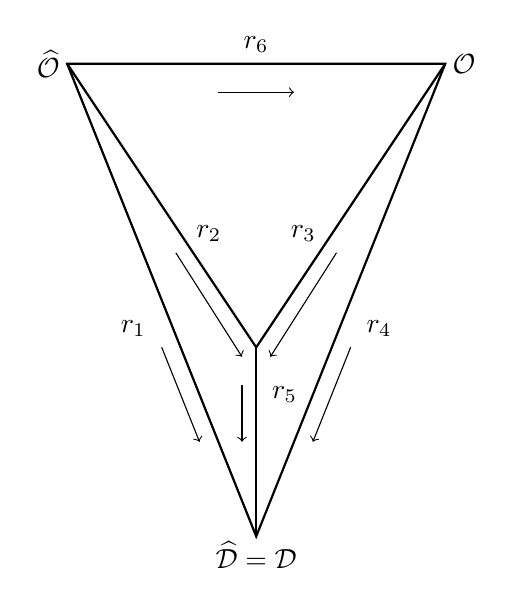
\begin{tikzpicture}[scale=1.2]

\coordinate (L) at (0,0);
\coordinate (R) at (4,0);
\coordinate (C) at (2,-3);
\coordinate (B) at (2,-5);


\draw[thick] (L) -- (R) -- (B) -- cycle;
\draw[thick] (L) -- (C);
\draw[thick] (R) -- (C);
\draw[thick] (C) -- (B);

\draw[->] (1.6,-0.3) -- (2.4,-0.3);

\draw[->] (1.15,-2) -- (1.85,-3.1);

\draw[->] (2.85,-2) -- (2.15,-3.1);

\draw[->] (1.85,-3.4) -- (1.85,-4);

\draw[->] (1, -3) -- (1.4, -4);

\draw[->] (3, -3) -- (2.6, -4);

\node at (0.7,-2.8) {$r_1$};
\node at (1.5,-1.8) {$r_2$};
\node at (2.5,-1.8) {$r_3$};
\node at (3.3,-2.8) {$r_4$};
\node at (2.3, -3.5) {$r_5$};
\node at (2, 0.2) {$r_6$};
\node at (-0.2, 0) {$\widehat{\mathcal{O}}$};
\node at (4.2, 0) {$\widecheck{\mathcal{O}}$};
\node at (2, -5.2) {$\widehat{\mathcal{D}} = \widecheck{\mathcal{D}}$};
\end{tikzpicture}
\quad
\]
La strada $r_6$ permette alla popolazione \textit{hat} di utilizzare anche le strade della \textit{check}.
Sempre riprendendoli da \cite[Cap. 3]{MR4911797}, usiamo i seguenti parametri:
\begin{equation*}
\begin{array}{r @{\hspace{2cm}} r}

\widehat{\tau}_1(\eta) = 4 &
\widecheck{\tau}_1(\eta) = +\infty \\

\widehat{\tau}_2(\eta) = 1+\widehat{\eta} &
\widecheck{\tau}_2(\eta) = +\infty \\

\widehat{\tau}_3(\eta) = +\infty &
\widecheck{\tau}_3(\eta) = \widehat{\eta} \\

\widehat{\tau}_4(\eta) = 5\widehat{\eta}+5\widecheck{\eta} &
\widecheck{\tau}_4(\eta) = 5\widehat{\eta}+5\widecheck{\eta} \\

\widehat{\tau}_5(\eta) = 1+\widehat{\eta}+\widecheck{\eta} &
\widecheck{\tau}_5(\eta) = 1+\widehat{\eta}+\widecheck{\eta} \\

\widehat{\tau}_6(\eta) = 1 &
\widecheck{\tau}_6(\eta) = +\infty 
$$
\end{array}
\end{equation*}
con:
\begin{equation*}
\begin{array}{r @{\hspace{2cm}} r}

\widehat{\gamma}_1 = r_1 &
\widecheck{\gamma}_1 = (r_3, r_5)\\

\widehat{\gamma}_2 = (r_2, r_5) &
\widecheck{\gamma}_2 = r_4 \\

\widehat{\gamma}_3 = (r_6, r_4) & \\
$$
\end{array}
\end{equation*}

Variando il costo della strada $r_6$ \textbf{solamente per la popolazione \textit{hat}}, da $\widehat{\tau_6}(\eta)=1$ a $\widehat{\tau_6}(\eta)=1.5$ otteniamo (vedi \autoref{script:20}):
\newpage
\vspace*{-4cm}

\begin{figure}[H]
\centering

\begin{tabular}{cc}

\includegraphics[height=6cm]{../figures/Es2/grafico_main_hat_Variazione_del_costo_delle_strade.png}&

\includegraphics[height=6cm]{../figures/Es2/grafico_main_check_Variazione_del_costo_delle_strade.png} \\


\includegraphics[height=6cm]{../figures/Es2/grafico_hat/hat_theta_1_Variazione_del_costo_delle_strade.png} &

\includegraphics[height=6cm]{../figures/Es2/grafico_check/check_theta_1_Variazione_del_costo_delle_strade.png} \\


\includegraphics[height=6cm]{../figures/Es2/grafico_hat/hat_theta_2_Variazione_del_costo_delle_strade.png} &

\includegraphics[height=6cm]{../figures/Es2/grafico_check/check_theta_2_Variazione_del_costo_delle_strade.png} \\


\includegraphics[height=6cm]{../figures/Es2/grafico_hat/hat_theta_3_Variazione_del_costo_delle_strade.png} &
\rule{0pt}{6cm} \\

\end{tabular}

\end{figure}
Come nella \autoref{subsec:Es1} osserviamo un Paradosso di Braess \cite{BraessParadox}. Questa volta, però, solo una delle due popolazioni
(\textit{check}) risente della variazione di costo di $r_6$, nonostante nessun veicolo \textit{check} la attraversi: l'aggiunta di $r_6$, che
non migliora il tempo di viaggio dell'unica popolazione che ne usufruisce (\textit{hat}), peggiora invece il tempo di viaggio dell'altra.

Nuovamente si nota che questo stato paradossale è solo localmente stabile: facendo variare, per esempio, il numero di veicoli nella popolazione \textit{check}, da $\widecheck{\zeta} = 1$
a $\widecheck{\zeta} = 6$ (vedi \autoref{script:21}):

\newpage
\vspace*{-4cm}

\begin{figure}[H]
\centering

\begin{tabular}{cc}

\includegraphics[height=6cm]{../figures/Es2/grafico_main_hat_Variazione_del_numero_di_individui_nella_popolazione.png} &

\includegraphics[height=6cm]{../figures/Es2/grafico_main_check_Variazione_del_numero_di_individui_nella_popolazione.png} \\


\includegraphics[height=6cm]{../figures/Es2/grafico_hat/hat_theta_1_Variazione_del_numero_di_individui_nella_popolazione.png} &

\includegraphics[height=6cm]{../figures/Es2/grafico_check/check_theta_1_Variazione_del_numero_di_individui_nella_popolazione.png} \\


\includegraphics[height=6cm]{../figures/Es2/grafico_hat/hat_theta_2_Variazione_del_numero_di_individui_nella_popolazione.png} &

\includegraphics[height=6cm]{../figures/Es2/grafico_check/check_theta_2_Variazione_del_numero_di_individui_nella_popolazione.png} \\


\includegraphics[height=6cm]{../figures/Es2/grafico_hat/hat_theta_3_Variazione_del_numero_di_individui_nella_popolazione.png} &
\rule{0pt}{6cm} \\

\end{tabular}

\end{figure}
Durante un transitorio iniziale del tempo di percorrenza la popolazione \textit{hat} 
smette progressivamente di utilizzare la $r_6$ e, nonostante la popolazione \textit{check} aumenti, il suo tempo di percorrenza rimane costante:
viene perso il comportamento paradossale della rete.